\documentclass[a4paper,12pt]{article}
\usepackage{times}
\usepackage[francais]{babel}
\usepackage[utf8x]{inputenc}
\usepackage[T1]{fontenc}
\usepackage{amsmath}
\usepackage{amssymb}
\usepackage{graphicx}
\usepackage{pdfpages}
\usepackage{pdflscape}
\usepackage{listings}
\usepackage{longtable}
\lstset{literate=
{é}{{\'e}}1
{è}{{\`e}}1
{ê}{{\^e}}1
{à}{{\`a}}1
{â}{{\^a}}1
}
\lstset{language=C++,
                basicstyle=\footnotesize,
                keywordstyle=\footnotesize\color{blue},
                otherkeywords={override,nullptr}
}
\definecolor{orange}{rgb}{0.8,0.4,0.0}
\definecolor{darkblue}{rgb}{0.0,0.0,0.6}
\definecolor{cyan}{rgb}{0.0,0.6,0.6}
\lstdefinelanguage{JSON}
{
  basicstyle=\normalsize,
  columns=fullflexible,
  showstringspaces=false,
  commentstyle=\color{gray}\upshape,
  morestring=[b]",
  morestring=[s]{>}{<},
  morecomment=[s]{<?}{?>},
  stringstyle=\color{orange},
  identifierstyle=\color{darkblue},
  keywordstyle=\color{blue},
  morekeywords={string,number,array,object}% list your attributes here
}

\sloppy

\setlength{\topmargin}{0cm}
\setlength{\headsep}{0.in}
\setlength{\headheight}{0.in}
\setlength{\evensidemargin}{0cm}
\setlength{\oddsidemargin}{-1cm}
\textwidth 18cm
\textheight 25cm

\begin{document}

\thispagestyle{empty}

\begin{titlepage}

\vspace*{2cm}

\begin{center}\textbf{\Huge Projet Logiciel Transversal}\end{center}{\Large \par}

\begin{center}\textbf{\large Auteurs}\end{center}{\large \par}

\vspace{2cm}

%\begin{figure}[h]
%\begin{center}
%\includegraphics[width=\textwidth]{exemple.png}
%\caption{\label{pacmangame}Exemple du jeu}
%\end{center}
%\end{figure}

\clearpage

{\small
\tableofcontents
}

\end{titlepage}

\clearpage

\section{Présentation Générale}

\subsection{Archétype}
Le jeu proposé se base sur Magic : The Gathering Online, la version numérique du jeu de carte à collectionner éponyme.

Dans Magic : The Gathering les joueurs assemblent un "deck" contenant au minimum 60 cartes et s'affrontent en utilisant celles-ci, Magic : The Gathering étant un jeu qui est séparé en deux étapes bien distinctes : la création de "deck" et le jeu de carte, nous nous focaliserons sur une seule de ces deux composantes : le jeu de carte.


\subsection{Règles du jeu}

\subsubsection{Glossaire}

Joueur actif : Joueur dont c'est le tour
Engagé/Dégagé : un permenant est dit engagé lorsque la carte qui le représente est tourné de 90 degrés vers la droite, il est dit dégagé lorsqu'il ne l'est pas. 

\subsubsection{Zones de jeu}
Le Jeu est composé de sept zones :

- La Bibliothèque : Chaque joueur a la sienne, c'est la zone ou les joueurs placent leurs "deck" faces cachés, lorsqu'un joueur pioche il pioche depuis cette zone.

- La Main : Propre à chaque joueur, c'est la zone depuis laquelle les joueurs peuvent jouer des cartes.

- Le Cimetiere : Propre à chaque joueur, c'est la zone ou les joueurs placent les cartes déffausés.

- L'exile : Propre à chaque joueur, c'est la zone ou vont les cartes retirés du jeu par des effets de cartes.

- Le champ de battaile : Commun a tous les joueurs, c'est la zone ou l'on trouve des permanents qui sont soit des cartes soit des "jetons" créer par des effets de cartes.

- La Pile : Commune a tous les joueurs c'est la zone ou vont les cartes jouées, effets de cartes et effets de permanents avant d'etre résolus.

- Zone de commandement : Commune a tous les joueurs, c'est une zone ou vont des objets qui ne pourront etre altéré par des effets de cartes.

\subsubsection{Condition de défaite}
Un joueur perd la partie si : 

-Ses points de vie sont réduits a zéro

-Il pioche alors que sa bibliothèque est vide

-Un effet de carte lui fait perdre la partie

-Un effet de carte fait gagner un de ses advairsaires 

\subsubsection{Structure du tour}
Le tour est composée de cinq phases : 
- Phase de début de tour : phase pendant laquelle le joueur actif pioche une carte et dégage les permanents qu'il controle.

- Phase principale : C'est la phase durant laquelle le joueur actif peut jouer des sorts "lent".

- Phase de combat : C'est la phase durant laquelle le joueur actif va déclarer une ou plusieurs créatures comme attaquant un autre joueur , le joueur défenseur pourra alors bloquer avec ses propre créatures.

- Phase principale post-combat : voir phase principale ci-dessus.

- Phase de fin de tour : C'est la phase durant laquelle le joueur actif va défausser des cartes s'il en a trop en main et où toutes les bléssures de combats sur les créatures sont retirées.

\subsubsection{Déroulement de la partie}
Chaque joueur commence la partie avec un total de vingt points de vie et une main de départ de sept cartes.
La partie commence dans la phase principale du premier joueur qui joue et à la fin de son tour le tour d'un de ses adversaires commence, cela continue jusqu'à ce qu'un joueur est gagné la partie.

\subsection{Ressources}



\clearpage
\section{Description et conception des états}

\subsection{Description des états}


\subsection{Conception Logiciel}


%\begin{landscape}
%\begin{figure}[p]
%
\includegraphics[width=0.9\paperheight]{state.pdf}
%\caption{\label{uml:state}Diagramme des classes d'état.} 
%\end{figure}
%\end{landscape}

\clearpage
\section{Rendu: Stratégie et Conception}

\subsection{Stratégie de rendu d'un état}


\subsection{Conception logiciel}

%\begin{landscape}
%\begin{figure}[p]
%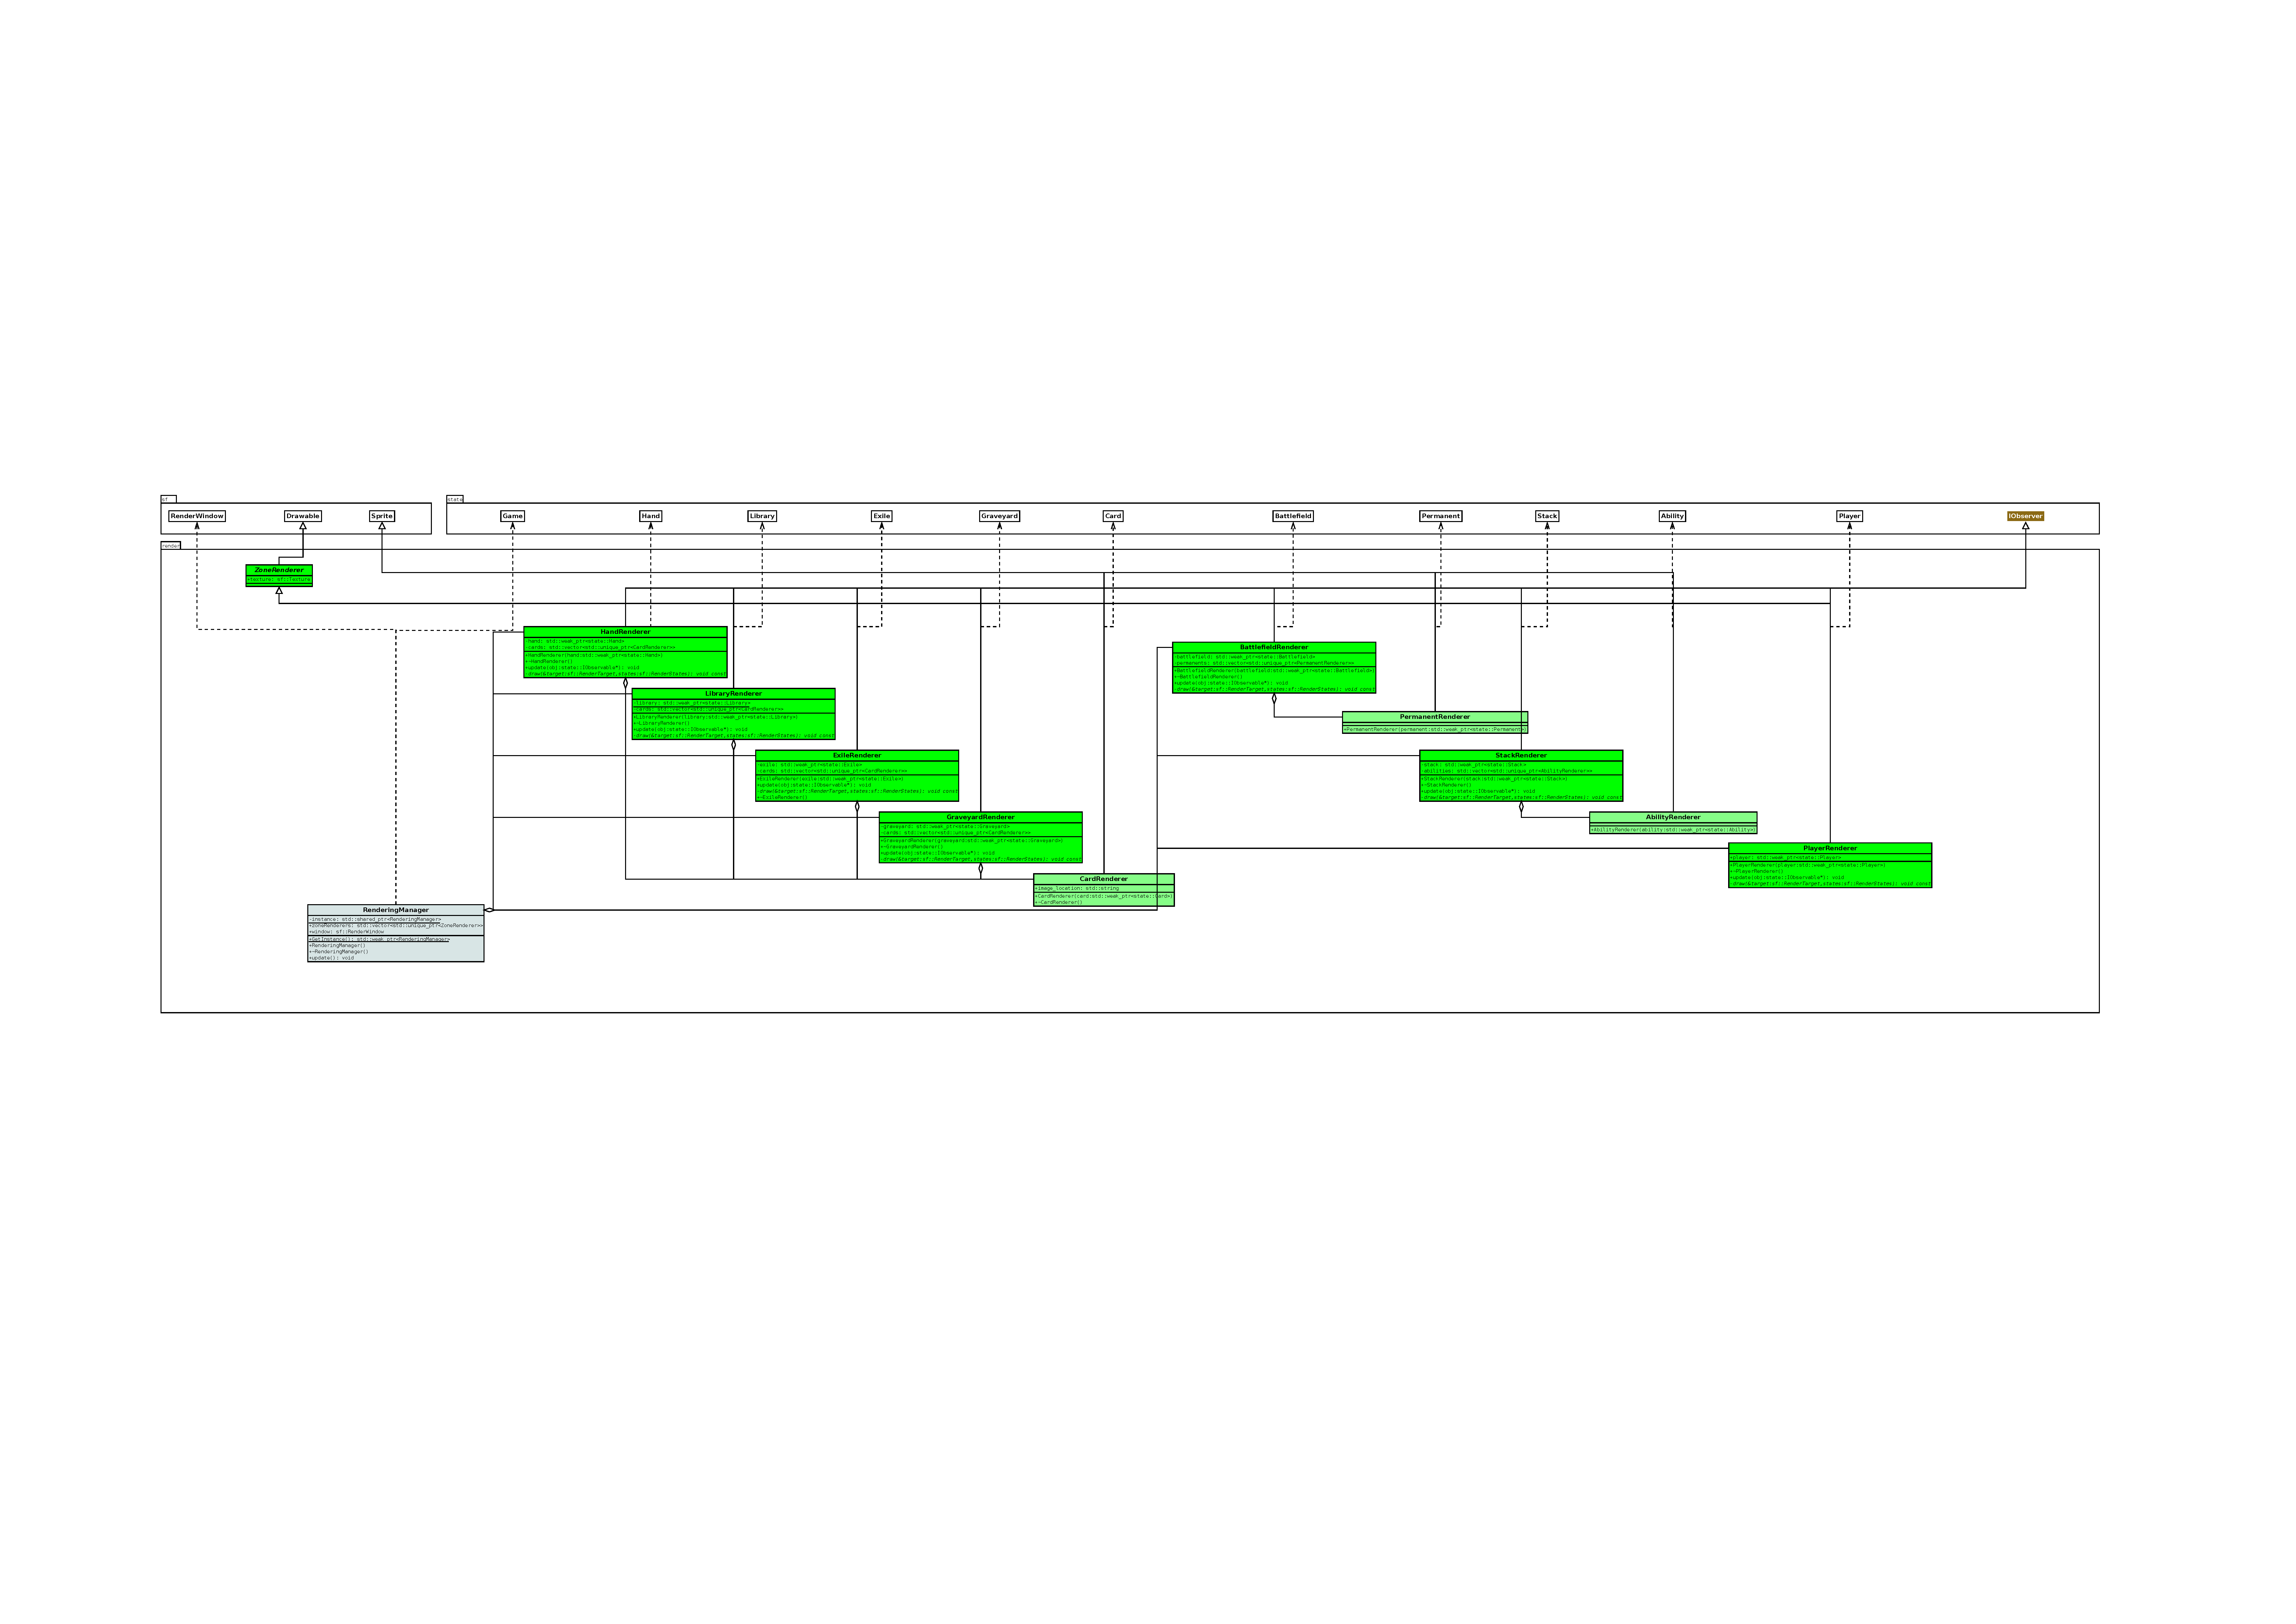
\includegraphics[width=0.9\paperheight]{render.pdf}
%\caption{\label{uml:render}Diagramme des classes de rendu.} 
%\end{figure}
%\end{landscape}

\clearpage
\section{Règles de changement d'états et moteur de jeu}

\subsection{Règles}

\clearpage
\subsection{Conception logiciel}


%\begin{landscape}
%\begin{figure}[p]
%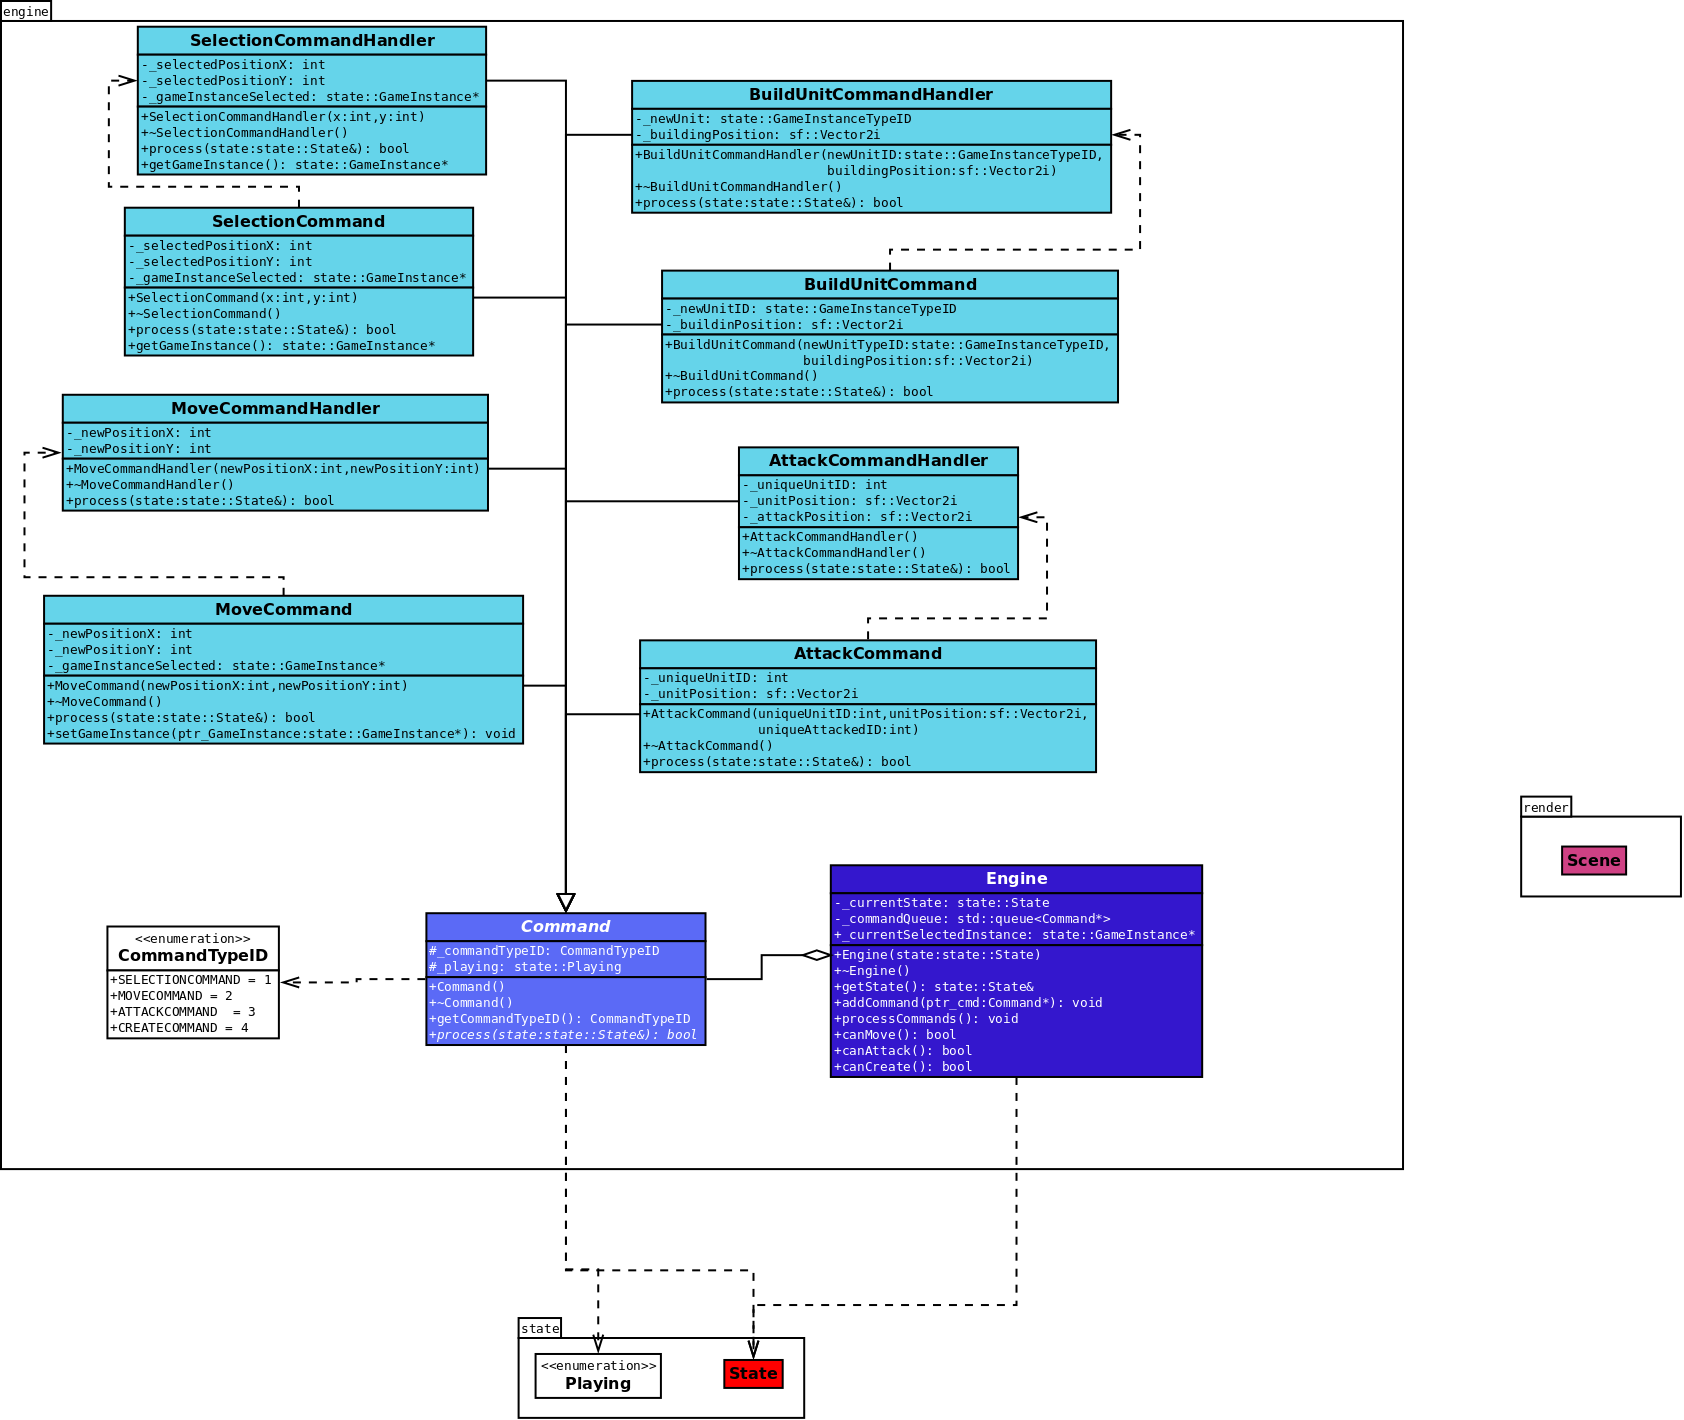
\includegraphics[width=0.9\paperheight]{engine.pdf}
%\caption{\label{uml:engine}Diagramme des classes de moteur de jeu.} 
%\end{figure}
%\end{landscape}


\section{Intelligence Artificielle}

\subsection{Stratégies}

\clearpage
\subsection{Conception logiciel}


%\begin{landscape}
%\begin{figure}[p]
%\includegraphics[width=0.9\paperheight]{ai.pdf}
%\caption{\label{uml:ai}Diagramme des classes d'intelligence artificielle.} 
%\end{figure}
%\end{landscape}


\section{Modularisation}
\label{sec:module}

\subsection{Organisation des modules}

\clearpage
\subsection{Conception logiciel}


%
%\begin{landscape}
%\begin{figure}[p]
%\includegraphics[width=0.9\paperheight]{module.pdf}
%\caption{\label{uml:module}Diagramme des classes pour la modularisation.} 
%\end{figure}
%\end{landscape}

\end{document}
